\documentclass[]{article}

%opening
\title{Malicious context and workaround analysis of decentralized VPN:\\the case of Mysterium Network}
\author{Jacopo Federici}


\usepackage{imakeidx}
\usepackage{setspace}
\usepackage{url}
\usepackage{graphicx}
\usepackage{listings}
\usepackage{array,multirow,graphicx}
\usepackage{float}
\makeindex

\begin{document}
	\raggedright
	\setstretch{1.0}
	\maketitle	
	\clearpage
	
	\tableofcontents{}
	\pagebreak

	\begin{abstract}
		
	\end{abstract}
	\pagebreak


	\subsection{Work structure}
	\subsection{Outline}
	\subsection{Goal}

	\section{State of the art}

	\subsection{Introduction}
	The need for privacy is becoming more critical day after day: the massive digitalization of many aspects of our life implicitly exposes us and our data and even the simplest operations which use an internet connection are becoming unsafe.\\
    In the last years, we have seen security solutions integrated into popular applications, such as browsers or mobile apps, following the increase of security attacks. For instance, in 2017, the popular Chrome browser announced it would mark as non-secure any website using the HTTP protocol instead of HTTPS. This move was to encourage the website to use SSL/TLS certificates and make secure the communication between client and server. It's interesting to discover the Netscape Navigator browser has made the first HTTPS version around 1990, but the official RFC publication has been released only in May 2000 \cite{HTTPS}.\\
	Similar scenario for the VPN: abbreviation for "virtual private network" it's a technical solution to extend a private network across a public network. It creates a virtual point-to-point connection through the use of a tunneling protocol over the existing network, and the tunneled traffic is encrypted. A first VPN specification proposal is around 2000 \cite{VPNRFC}, but only in the last years, the use of VPN became massive. The VPN data encryption feature is solving privacy problems that only lately are beeing relevant. Those problems can be exiting a censored network, using services available or blocked in certain countries, avoiding tracking methods and other similar scenarios.\\
	Currently, there are commercial solutions that allow users to have a private connection to the company's servers across the world, but there are many security concerns about those solutions. The company can keep the connection logs, inspect the traffic, or sell statistical data.\\
    Some open-source projects were, lately, born to solve these problems. Their goal is to revolution the idea of VPN and its uses, building a rich network of peers where two nodes can connect through a VPN. The project provides a platform that includes all the components needed to have an efficient, fast, and easy-to-use system: from the discovery to the payment.\\
    
    In this research document, we analyzed the most developed project, Mysterium Network, as a case of study. As we write, Mysterium offers a working network composed of hundreds of nodes around the world, making it the best project to investigate malicious contexts and design vulnerabilities on, owns by the decentralized architecture, more than the Mysterium project itself.\\
	We even discover how secondary aspects are pivotal to guide attacks to the system.\\
    The second step focuses on the solutions that can patch those critical aspects and provides a comparison of them with an eye on the practical perspective.
	
	\subsection{The world now}
	We are still in the middle of a large transformation. From the invention of the pc and the birth of the internet, more and more services are becoming digital; more and more people are using those services; more and more bad guys are trying to pull down those services.\\

	But there are differences from some decades ago.\\
	First, everything is now much faster. The internet infrastructure allows us to move significant amounts of data within a few seconds. Furthermore, our personal computer can perform operations that were impossible to execute some years ago on mainstream servers. This speed is jeopardizing many security solutions, such as ciphers that based, and still base, their strength on the practical difficulties to solve the mathematical problems at the base of cipher methods.\\
	Second, the architecture is moving back to a cloud-based infrastructure. Many workflows see, again, a thin client sending the execution step to a cloud server that elaborates the output that is then sent back to the client. This architecture changes the surface of the attack targeting the cloud servers as the principal attack destinations.\\
	Third, some technologies are mature enough to provide an excellent alternative to traditional models — for instance, the cryptocurrency model against the bank model. Here, the changes regard the paradigma, and the reasons behind these new approaches are much more than technological.\\

	\textit{The security noun is changing the meaning inside the people's minds, from "how thick is my bank caveau" to "how long my bank requires my new online account password"}

	\subsection{the need for trust and privacy}

	\begin{verbatim}
		https://www.geeksforgeeks.org/need-of-information-security/
		https://www.hackerfactor.com/blog/index.php?/archives/868-Deanonymizing-Tor-Circuits.html
		https://www.howtogeek.com/133680/htg-explains-what-is-a-vpn/
		https://www.forbes.com/sites/tjmccue/2019/06/20/why-use-a-vpn/#3f08d7105859
		https://www.investopedia.com/terms/b/blockchain.asp
		https://www.howtogeek.com/350322/what-is-ethereum-and-what-are-smart-contracts/
		
		https://en.wikipedia.org/wiki/Proof_of_work
		https://en.wikipedia.org/wiki/Proof_of_stake
	\end{verbatim}

	Anonymization: in every network systems, anonymization is a tough challenge. Even more, if privacy is a crucial point. In some countries, the VPN is massively used to protect data from surveillance at any level, from a public unsecured wifi connection to the country ISPs.\\There are countries, the People's Republic of China for example, where censorship is present and where identity obfuscation is, therefore, necessary to protect yourself. In these cases, the use of a VPN is a solution, as long as a safe company provides it. With the adjective `safe' we mean a company that does not make you or your traffic detectable or even worsts sniffs and crafts your data for malicious actions.\\

	The decentralized VPN completely changes the paradigma, the design of the infrastructure.\\
	An analogy can be made with the traditional bank model: as we know, the bank is a centralized entity trusted by definition. What if the bank suddenly becomes untrusted? Cryptocurrencies spread among ourselves, the cryptocurrency owners, and network participants the trusts we put in the bank, using a blockchain as a technical solution. 
	A similar design is used with decentralized VPN: there is no central entity to control the system, but a significant number of peers, the network, we can choose to connect.

	\subsection{We are our trust}

	\subsubsection{Decentralized VPNs}

	A decentralized VPN is a network of nodes where the users can connect through a VPN to nodes without a central entity. The decentralization system, in this context, includes several steps to make the final connection happening, rather than a simple VPN connection between two peers.\\
	First of all, the user creates an identity into the system, linked to the payment wallet, using a client application. Then, he connects to the network providing his availability to be a consumer or a provider.\\
	The consumer user chooses the provider he prefers based on different features such as the region, quality, or cost of the node, and asks for a new connection to that server. In this step, the blockchain, based on Ethereum, allows creating a smart contract between the two participants with a predetermined amount of money. Using commercial VPN applications, such as OpenVPN or Wireguard, the connection between consumer and provider, otherwise called client and server, is established. When the connection correctly ends, the network closes the smart contract, that registers the result of the transaction in the blockchain.\\
	We outlined the main steps from which we can think of a decentralized VPN more as a platform solution rather than a simple VPN application. Indeed, other projects suggested the VPN is one of the features a decentralized system so composed can have. (EXPLAIN BETTER THE IDEA)  
		          
	\subsubsection{The business idea}
	As a business project, which aims to earn money, the project has a specific business plan: provide a system network where users can join as a service provider, selling their internet bandwidth, or as a service consumer, buying other's internet bandwidth. For every cryptocurrency transaction, the network applies a fee that wants, substantially, to create a market to manage.\\
	Each couple of entities, a consumer and a provider, agree on a transaction paid using cryptocurrency in the face of the used service. This transaction is regulated by an Ethereum smart contract signed by both sides and requires a fee to be closed. This fee is not the Ethereum fee, generally called gas, but the precisely Mysterium source of earnings. For this reason, Mysterium and other projects created their coins used to buy and sell internet bandwidth between the nodes inside the network. The coin name is MYST for Mysterium Network and, as a regular cryptocurrency, it is possible to convert MYST to ETH and vice versa.\\
	Although a node can decide to be a consumer or a provider at any moment, the two entities are different, and the type of market is called a two-sided market where bid and ask respectively grow on the other side growth. (EXPLAIN BETTER)\\

	\begin{verbatim}
		concetti introduttivi
		- blockchain in linea di massima\\
		- ethereum in linea di massima e descrizione degli smart contracts\\
		- proof of work, proof of stake\\
		- reputazione in una net (Eigentrust)\\
		- - cercare applicazione pratica di Eigentrust\\
		- descrizione di BFT\\
	\end{verbatim}
	
	\section{Mysterium Network}
	
	The main open-source projects which aim to create a decentralized VPN are Mysterium Network, Privatix, Substratum, and Sentinel. We explored all of them, and we can safely say the most advanced project is Mysterium Network, at the time we are writing this research document.\\It is the most completed in terms of development and design. Furthermore, it's 100\% open source, that for this kind of project is a requirement which conditions the users' adoption and the market diffusion.\\
	Therefore, we decided to use the Mysterium Network as a test case to analyze the malicious context the project is exposed to and propose our proof of concepts as solutions.
	
	\subsection{Architecture}
	Mysterium Network is an open-source project. Its main goal is to build a decentralized infrastructure made up of layered VPN protocols, blockchain, and smart contracts.\\
	As described in figure X, we can distinguish between a service client block and a service provider block. Both of them lean on the Ethereum blockchain block, which is a distributed database where all the network operations, the identities, and the service proposals are recorder.\\

	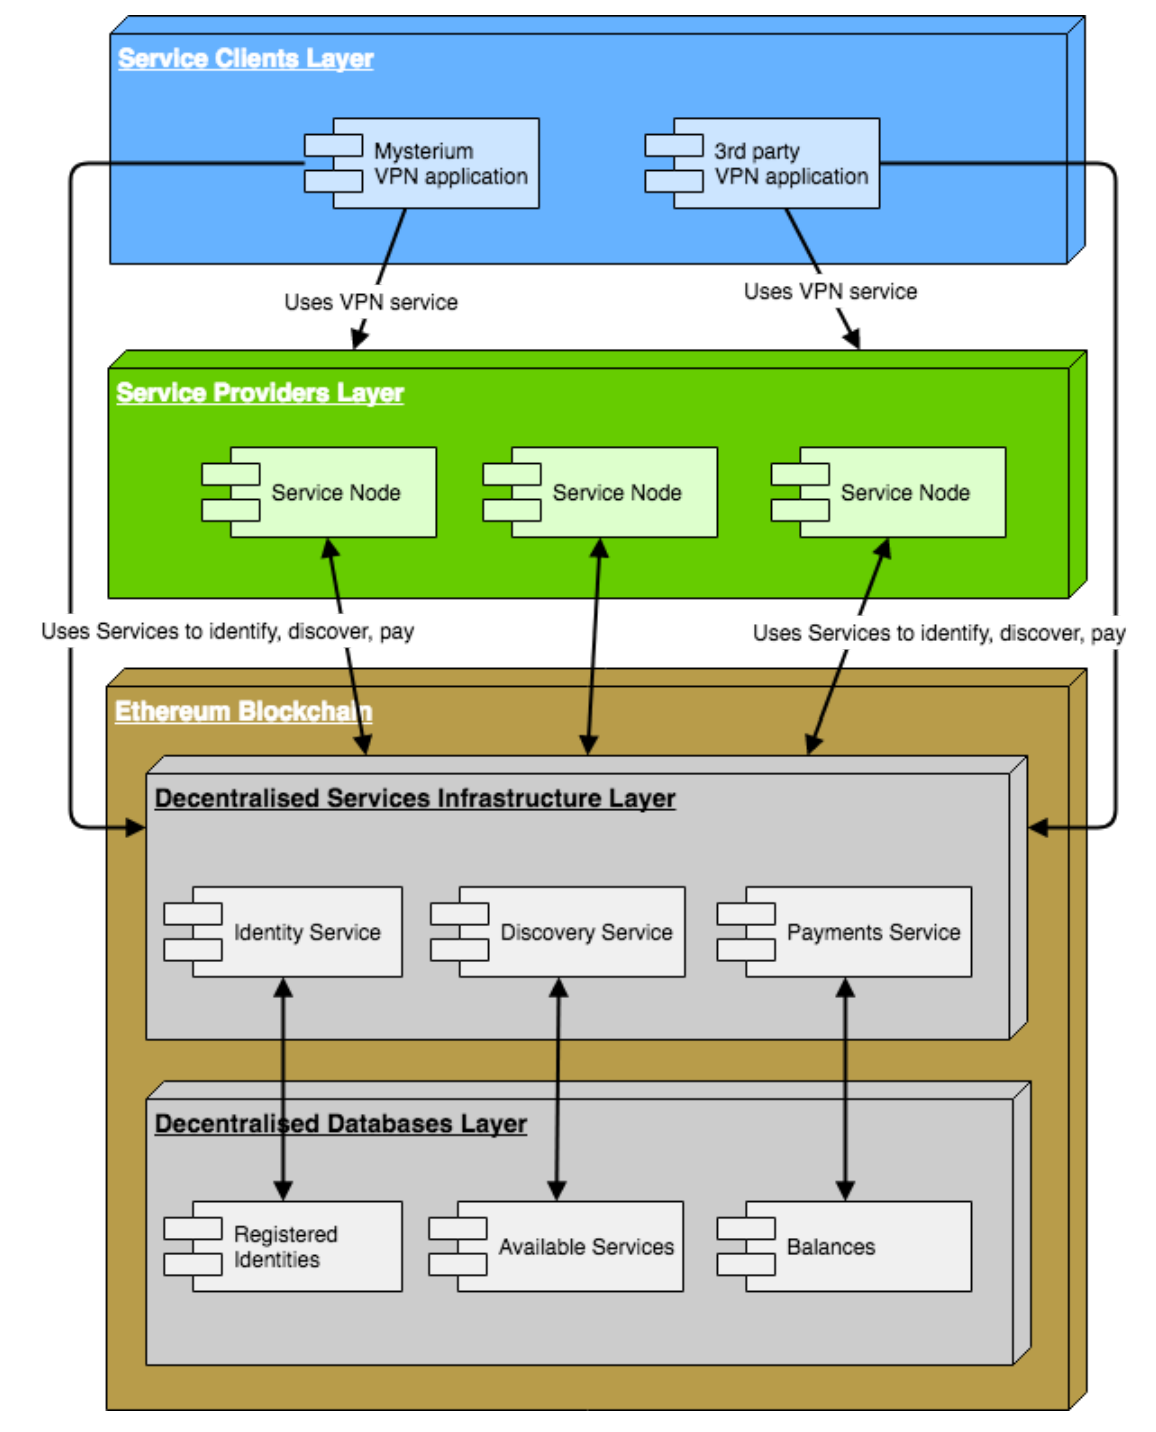
\includegraphics[width=0.5\linewidth]{"images/mysterium_architecture.png"}
		
	As a general workflow description, Mysterium starts by collecting all the agents' service proposals and presents them to the clients. Then it registers the client's intention to pay for the agent's service chosen by the user and creates the VPN connection between the two points. The outcome of each transaction is saved in the blockchain.\\
	
	To implement all the functionalities just said, Mysterium has four core components inside its architecture:
	\begin{itemize}
		\item \textbf{Ethereum Blockchain} allows running decentralized code with smart contracts, enabling reliable services and payment handling.
		\item \textbf{Identity service and database of registered identities} ensure the proper identity acknowledgment between client and service provider.
		\item \textbf{Discovery service and database of available services} provide means to announce the availability of VPN services and to pick the most suitable VPN service.
		\item \textbf{Payment service and database of balances} allow secure promise-based micropayments for services.
	\end{itemize}

	\subsubsection{Identity Service}

	The \textbf{identity service} manages the network identities that every node needs. A single node can create one identity or more, and each of them consists of a public and a private key. The last 20 bytes of the hash function, applied on the public key, is the unique id used to identify the node into the network. To publish a new identity so that other network members can reach it, Mysterium uses the smart contract mechanism. The private and public keys are used to validate the signature for the communication between the nodes.\\
	The blockchain mining process appends the public key and the unique id to the Ethereum blockchain after the node pays a fee to the network. This amount of money has the purpose of giving value to the identity. In such a way,  to abandon the identity to create a new one is unattractive, because it is expensive, but not impossible.\\ 
	We will discuss those aspects later, but we can surely say this is the first barrier to block in mass identity creation.\\
	Furthermore, the user benefits in using the same identity because it is possible to rebuild his transaction history and his balance from the Ethereum blockchain, making the user more predictable and thus trustworthy for service providers.\\

	\begin{figure}
		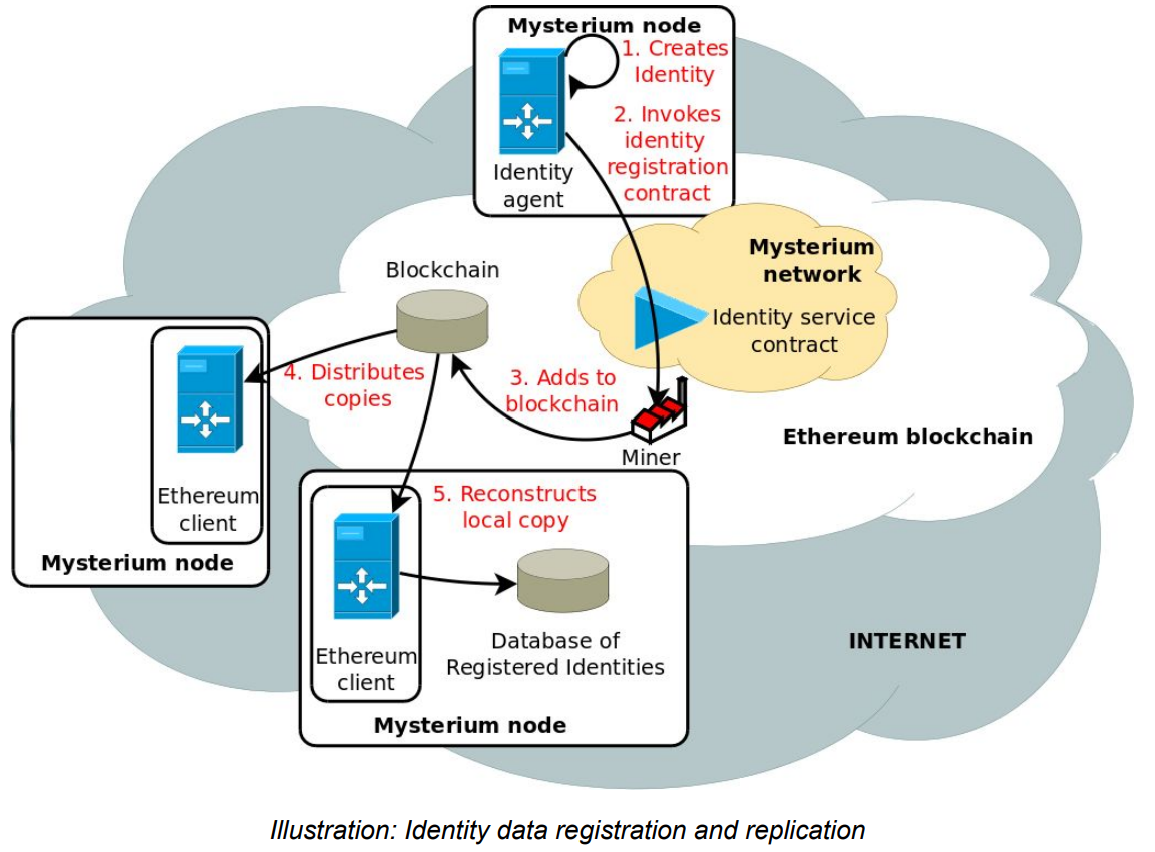
\includegraphics[width=0.5\linewidth]{"images/mysterium_identity_creation.png"}
		\caption{The Mysterium identity creation steps}
	\end{figure}

	\subsubsection{Service Discovery}

	The \textbf{service discovery} provides the list of service proposals available in the network. The service posts its service offer characterized by some service parameters: those parameters can be the VPN application the provider supports, the provider's connection IP address and port, the provider's server location, or the bandwidth per session. Then, the miners append the proposal to the blockchain, making it publicly available for everyone.\\

	\begin{figure}
		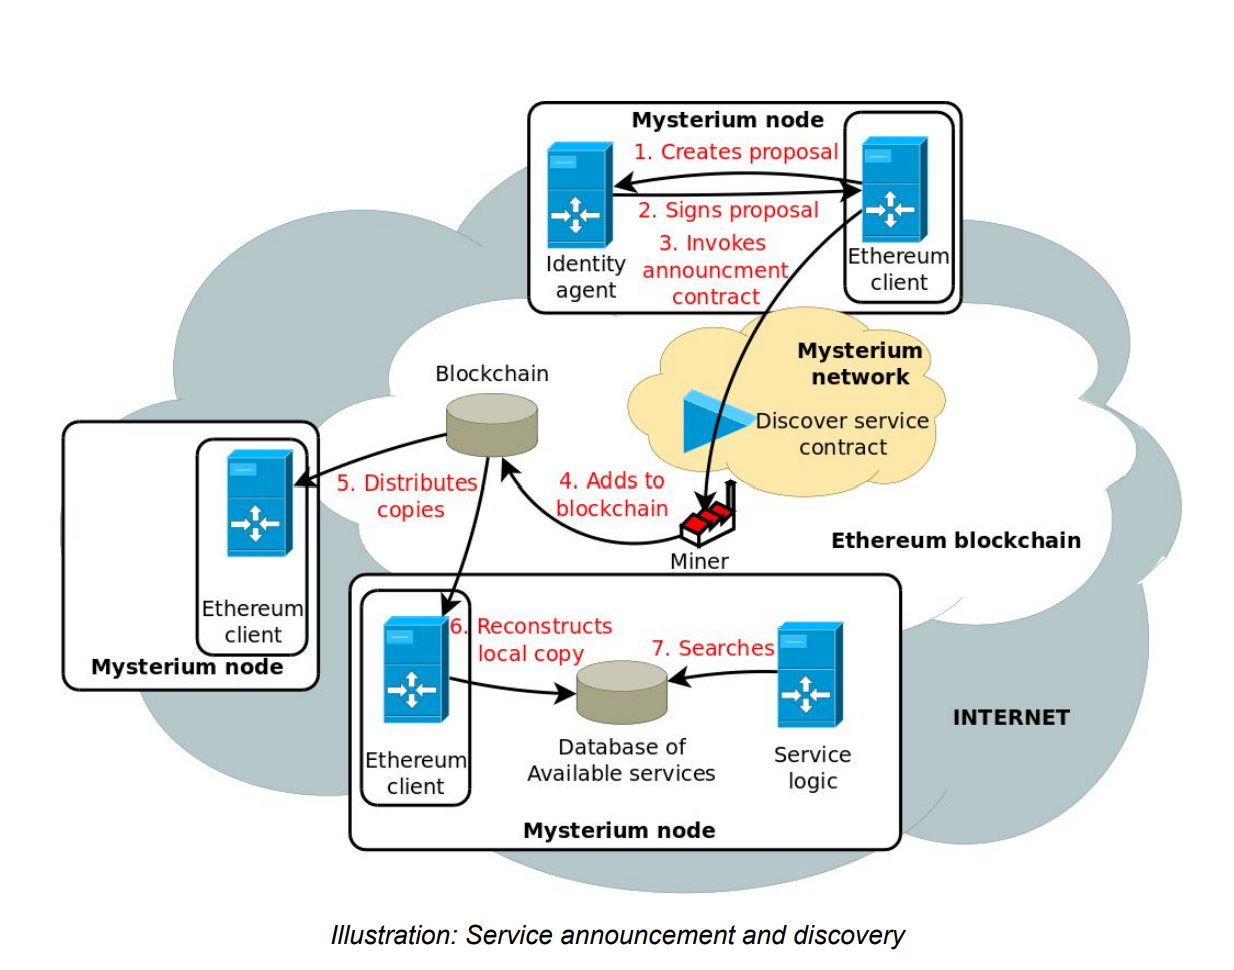
\includegraphics[width=0.5\linewidth]{"images/mysterium_service_announcement.png"}
		\caption{The Mysterium service announcement steps}
	\end{figure}
	
	\subsubsection{Payments Handling}

	Ethereum blockchain holds all the mechanisms for the \textbf{payments handling}. Therefore everyone needs an account to operate in the Mysterium Network. To advance a request, the consumer has to deposit currency in his wallet. Then, he can ask for a connection to a provider who has previously published a service proposal. Mysterium describes this step as a promise creation because the client effectively promises he will pay when the service ends. Positively clearing a promise is the everybody's best interest, the producer and the consumer, since a canceled promise marks the consumer's history hitting his reputation for future connections.\\
	From what we have described so far, it seems the consumer can decide to avoid paying for the used service: technically, it is possible, but realistically there are some considerations to be made.\\
	First of all, as previously described, identity creation takes money to be completed, and for any new connection, the user's balance has to be positive. In any case, the blockchain records any connection result so that everybody can rebuild the user's history at any moment. Therefore, it is possible to deduct the user's reputation based on its history.\\
	Using this reputation, the provider can decide to block his service to all users that have a low reputation caused by an unpaid precedent. On the other hand, other providers allow new users' connections with a low reputation but at a high price, accepting the risk of having an unpaid transaction.\\
	
	\subsection{Components}

	The core application is called \textbf{node}. It's written in GoLang, a new program language made by Google that is having a high adoption in the last years. The node creates a local webserver to connect to the network, manages the cryptocurrency wallet, and initiates the VPN connection as a client or manages the incoming connection as a server. Mysterium leans on famous VPN applications, which are OpenVPN and Wireguard.\\
	The node can be run in two modes, as a client or as a server, and it is managed via command-line interface or RESTful API, called TequilaAPI, exposed in the localhost.\\
	The main functionalities of TequilaAPI concern:
	\begin{itemize}
		\item the authentication,
		\item the connection,
		\item the identities,
		\item the location,
		\item the proposals,
		\item the service operations in provider mode
		\item other minor features
	\end{itemize}
		
	TequilaAPI is used by the client's application to manage the connection and for diagnostic operations.\\
	Mysterium developed a desktop client written using Electron, which uses the TequilaAPIs.\\
	The node is also available as a ready-to-use Docker image and published on the Docker Hub.\\
	On the mobile side, Mysterium is present with its multiplatform app that works only as a client.\\
	(MORE ON MOBILE)

	\subsection{setup}

	We have chosen the Linux platform and OpenVPN as the VPN application, but similar considerations can be made with different configurations.\\
	When the Mysterium application starts, it calls OpenVPN, which sets up its network environment. OpenVPN creates a virtual network device used to encrypt and decrypt the traffic. These devices reside in the kernel and are entirely virtual, which means there is no hardware on their back.\\They can be of two types, TAP or TUN.\\
	The TAP type is used to simulate a link layer device, which means the corresponding ISO model level it refers to is the number 2. Therefore, a TAP interface handles the transmission of the data frames between two nodes on the same physical layer. The behavior is equal to a bridge device: to connect two separates networks as if they were one.\\
	On the other hand, the TUN type is, in the ISO model, one layer above, working at level 3. A TUN interface handles packets, such as Internet Protocol packets. The main functions include port forwarding, host addressing, and traffic control, for example. The behavior is, in this case, equal to a router device: to connect two separates networks allowing their communication but keeping them independent.\\
	Usually, the TUN type is the most used, since the TAP type brings some limitations such as it cannot be used with Android or iOS devices, causes higher overhead on the VPN tunnel, and scales poorly.\\
	The following schema describes an example of a scenario where the network has two ethernet cards, one public and one internal.\\
	The virtual TUN interface created by OpenVPN is tun0, the public interface is eth0, and the internal interface is eth1.\\

	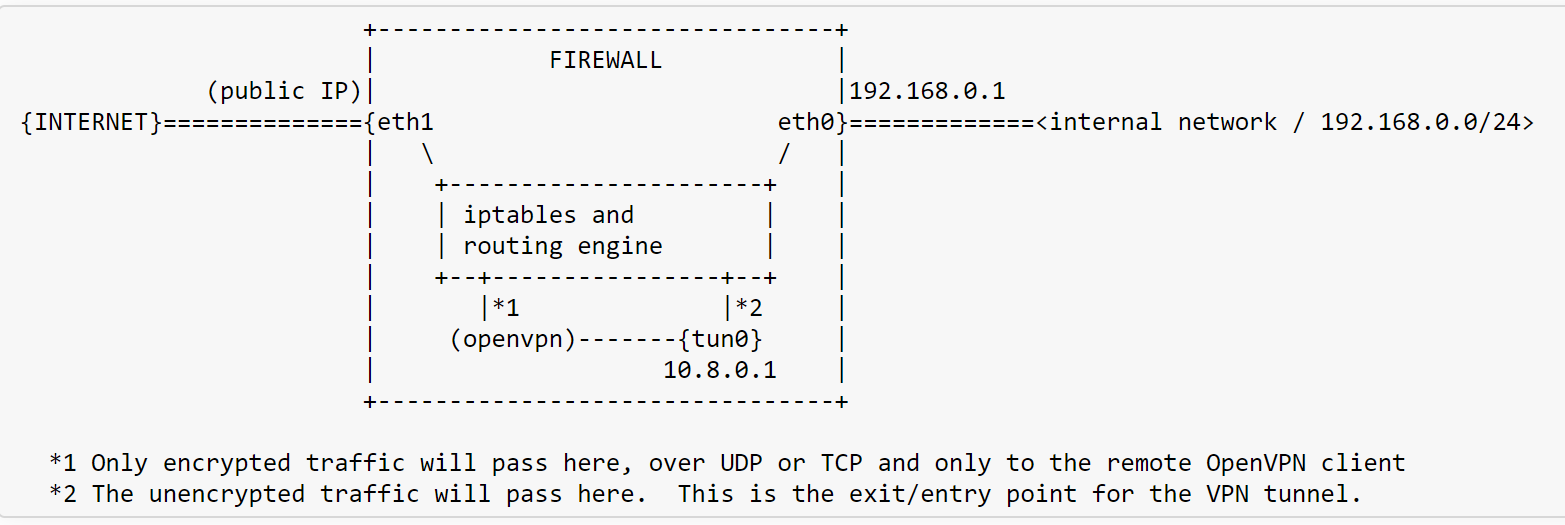
\includegraphics[width=1\textwidth]{"images/openvpn_routing_setup.PNG"}

	When a packet arrives at the eth1 interface, OpenVPN picks it up, decrypts, and sends the data to the tun0 interface. The ``iptables'' and the routing engine filter and masquerade the packet and send it to eth0, where it becomes available to the final receiver.\\On the other direction, when a packet arrives at eth0 interface, ``iptables'' and the routing engine apply their rules to filter and masquerade and then forward it to tun0 interface. Then, OpenVPN picks it up, encrypts the data, and sends it to the public eth1 interface.\\
	In our scenario, the network configuration is slightly different and does not include an internal interface network. As the schema below describes, OpenVPN sends traffic coming from ``tun0'' to the public interface eth0 on a specific port. The client application listens on that port the traffic that its OpenVPN client decrypts. \\

	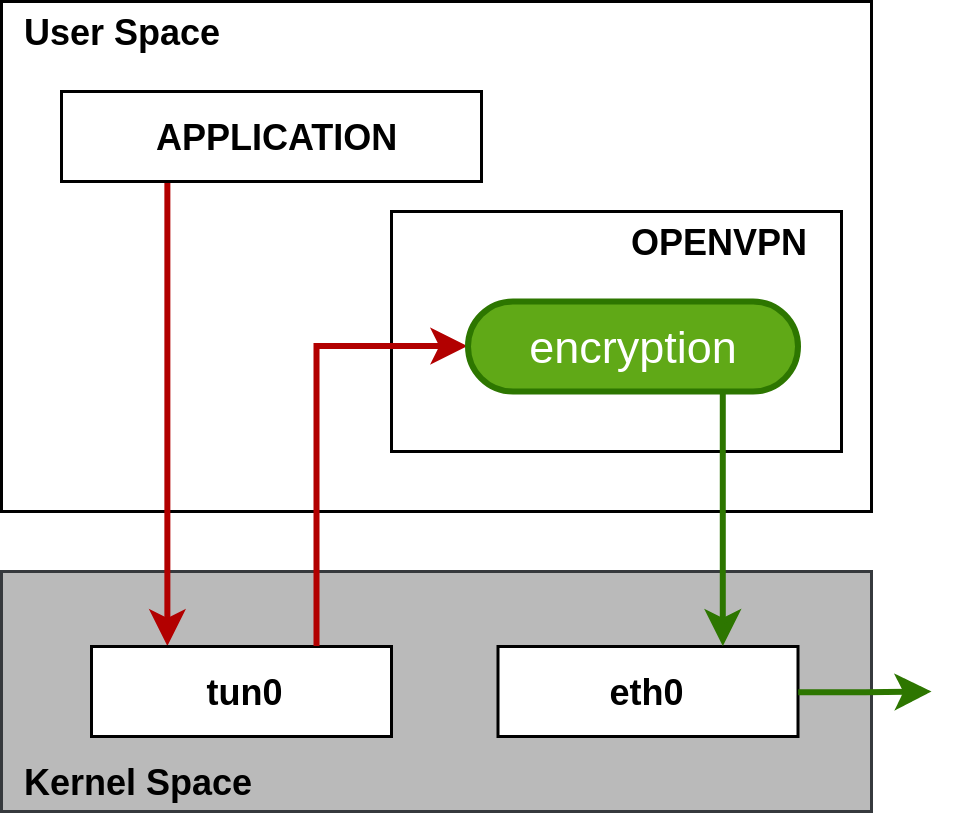
\includegraphics{"images/openvpn_tun_interface.jpg"}
	IMAGE TO EDIT AS BEFORE DESCRIBED\\

	\subsubsection{iptables}

	The ``iptables'' is a framework to manage the network decisions. It is based on the ``Netfilter'' kernel component, which exposes a set of hooks that are triggered at specific points of the network stack. Every packet that enters the networking system will trigger these hooks as it proceeds through the stack so all the programs that register with these hooks can interact with the traffic.\\
	Five different hooks correspond to different points of the stack:\\

	\begin{itemize}
		\item \lstinline{NF_IP_PRE_ROUTING}
		\item \lstinline{NF_IP_LOCAL_IN}
		\item \lstinline{NF_IP_FORWARD}
		\item \lstinline{NF_IP_LOCAL_OUT}
		\item \lstinline{NF_IP_POST_ROUTING}
	\end{itemize}

	IMAGE OF THE POINTS IN THE FLOW WHERE THE HOOKS ARE
	
	Iptables is substantially a firewall which organizes its rule in tables and chains. The tables classify the rules according to the type of decision that regards the packet.\\
	The available tables are the filter table, the NAT table, the Mangle table, the Raw table, and the Security table.\\
	The chains correspond to the available hooks, therefore iptbales has the \textbf{prerouting}, \textbf{input}, \textbf{forward}, \textbf{output}, and \textbf{postrouting} chains.\\
	The following table explains the triggering logic and execution precedence.\\

	\begin{tabular}{|l|c|c|c|c|c|}
	\textbf{\begin{tabular}[c]{@{}l@{}}Chains\\ Tables\end{tabular}} & \rotatebox[origin=c]{90}{\textbf{PREROUTING}}    & \rotatebox[origin=c]{90}{\textbf{INPUT}}         & \rotatebox[origin=c]{90}{\textbf{FORWARD}}       & \rotatebox[origin=c]{90}{\textbf{OUTPUT}}        & \rotatebox[origin=c]{90}{\textbf{POSTROUTING}}   \\\hline
	\textit{ruoting decision} & & & & X & \\\hline
	\textbf{raw} & X & & & X & \\ \hline
	\textit{connection tracking enabled} & X & & & X & \\\hline
	\textbf{mangle} & X & X & X & X & X \\\hline
	\textbf{DNAT (NAT)} & X & & & X & \\ \hline
	\textit{routing decision} & X & & & X & \\ \hline
	\textbf{filter} & & X & X & X & \\ \hline
	\textbf{security} & & X & X & X & \\ \hline
	\textbf{SNAT (NAT)} & & X & & & X
	\end{tabular}

	The packet triggers the hooks from the first row going down to the bottom of the table. It enters the chain depending on the routing decisions that are made, on its direction, incoming or outgoing, and whether the filtering rule accepts the packet.\\

	The chain traversal order is the following:
	\begin{itemize}
		\item Incoming packets destined for the local system: PREROUTING - > INPUT
		\item Incoming packets destined to another host: PREROUTING - > FORWARD - > POSTROUTING
		\item Locally generated packets: OUTPUT - > POSTROUTING
	\end{itemize}
	
	Every chain is a list of rules. Every packet is checked against each rule and, if the matching component checks, iptables executes an action.\\
	The rule can match the packet depending on the protocol type, the source or destination address, or packet, among other criteria.\\
	The action called target, which is triggered if the rule matches, can be of terminating or non-terminating type.\\
	The terminating type target causes the packet to exit the chain after a verdict that can be to allow or to drop the packet. The non-terminating type target causes the packet to continue its evaluation in the chain. There can be any number of non-terminating targets before a terminating one.\\
	A very used non-terminating target is the jump action: a rule can decide to jump a packet into another chain, and when that chain finishes the rules check, the execution comes back to the previous chain. This way is useful to organize the rules in chains based on their purposes.\\

	LITTLE IMAGE OF CHAIN JUMP ACTION

	\subsection{Design vulnerabilities}

	Mysterium is a complex system that integrates components of different types. The distinct nature of these components and their conjunction opens to new vulnerabilities scenarios and focuses on how the elements dialog each other.\\
	In the following chapter, we provide detailed considerations on Mysterium Network, but we faced some limitations: the Mysterium project is still under development, and they plan a full decentralized network will only in 2021. For this reason, the analyzes that regard components not yet implemented, like the payment system, are only theoretical. (!!!) 

	There are several aspects that on a project like Mysterium must be considered to evaluate its design vulnerabilities.\\
	We classify them based on:
	\begin{itemize}
		\item the position in the network: the starting point, the endpoint or the middle point;
		\item the step of the complete flow: the service proposals, the promise issuing, the transaction closing, and others;
		\item the type of traffic manipulation: sniffing, filtering or crafting the data;
		\item side channels attack and other particular scenarios.
	\end{itemize}
	
	\subsubsection{The position in the network}

	In the simplest configuration, the network includes a starting point that is the service consumer node and an endpoint, which is the service provider node. The VPN tunnel connects the two nodes and encrypts their traffic. The service node, as previously described, is the consumer's exit point to the internet.\\
	We consider secure the traffic passing through the VPN tunnel because it is encrypted, while not secure the traffic outside the VPN, that is from the provider to the internet.\\
	The exit nodes connect two areas with two different security levels: for this reason, it is sensitive by default.\\
	There is a similar problem for the Tor network. Tor, which stands for The Onion Router, is a network of peers where the user's encrypted traffic is sent into, and it bounces multiple times before getting an exit node from where, finally, it reaches the external resource.\\
	(MAYBE DESCRIBE WHY MYSTERIUM AND TOR ARE DIFFERENCES)
	The traffic is encrypted for each bouncing, except the last one, where it must be in clear to connect to the internet resource. The last node's role is to decouple the encrypted network from clear internet, and this makes it so valuable. If an exit node is malicious, it can potentially understand all the data passing through it and going to the internet resource. A Sweden researcher, Egerstad \cite{exitnodeTOR}, in his research, intercepted thousands of emails, setting up malicious exit nodes around the world and sniffing the connection between his nodes and the clear internet.\\
	Another research found existing malicious nodes in the Tor network with a simple test. They built up a website with a login and a system to count the login attempts. Then, they used multiple Tor paths with different exit nodes to reach the page and try to access it. The system counted more login attempts that the researched have done: this means the exist nodes sniffed the connection and tried to login by themselves.\\
	
	In both cases, the use of HTTP instead of HTTPS was crucial. The final goal was to demonstrate the importance of the exit nodes. As we will discuss in the conclusions, to solve this kind of problem is necessary to add another security layer over the Tor or Mysterium networks.  







	In this configuration, as described by the following image, the provider can see all the passing traffic, both incoming and outgoing, performing all the manipulation he wants. We will discuss further this scenario analyzing the technical solutions and providing a practical example to exploit, but, at first glance, this design vulnerability is unavoidable. \textit{If we ask someone to look at a photo for us and tell us to describe its content, he must, of course, understand the meaning, can change a little detail, or even tells someone else the content of the picture.}\\
	
	An improved configuration has one or more middle points between the consumer and the provider. Those points are called hops, and they act similarly to the provider node since they forward the traffic.\\
	These hops are nodes that manage encrypted data because they are inside the VPN tunnel, so they do not understand the data meaning. The vulnerabilities, in this scenario, are restricted to all the operations that concern the traffic shape, with no abilities to understand it. These actions hit the quality of service, a class of attacks that aim to lower or even block the service.\\
	For example, a middle node can slow down the data speed that it forwards. This operation is as simple as fast and does not need to understand the content at all. It can be made with a Linux package called ``tc'' \cite{tc} that stands for Traffic Control.\\

	\begin{verbatim}
		sudo tc qdisc add dev eth0 root netem delay 500ms
		# and turn it off with
		sudo tc qdisc del dev eth0 root netem
	\end{verbatim}

	With this command, every packet sent to the interface eth0 has a delay of 500 milliseconds.\\
	In this simple way, the traffic speed between the consumer and the provider has a poor quality because one or more middle points are performing this slowing down the operation. From the consumer side, the poor connection is a quality agreement breach, and it affects the service provider's reputation. Since the provider can detect the slow speed, he can suppose it is a packet path issue and can propose to the network to change one or more middle nodes. 

	\subsubsection{The flow steps}
	The first and easiest idea to implement to use the system maliciously has already been presented before: the attacker is the consumer, he creates an account in the Mysterium Network, has a positive balance to the cryptocurrency wallet, and look for a service proposal. They agree on the service cost and issue a payment promise. If the user does not respect the promise...




	\subsubsection{Traffic manipulation}





	\subsubsection{Side channels attack and particular scenarios}


	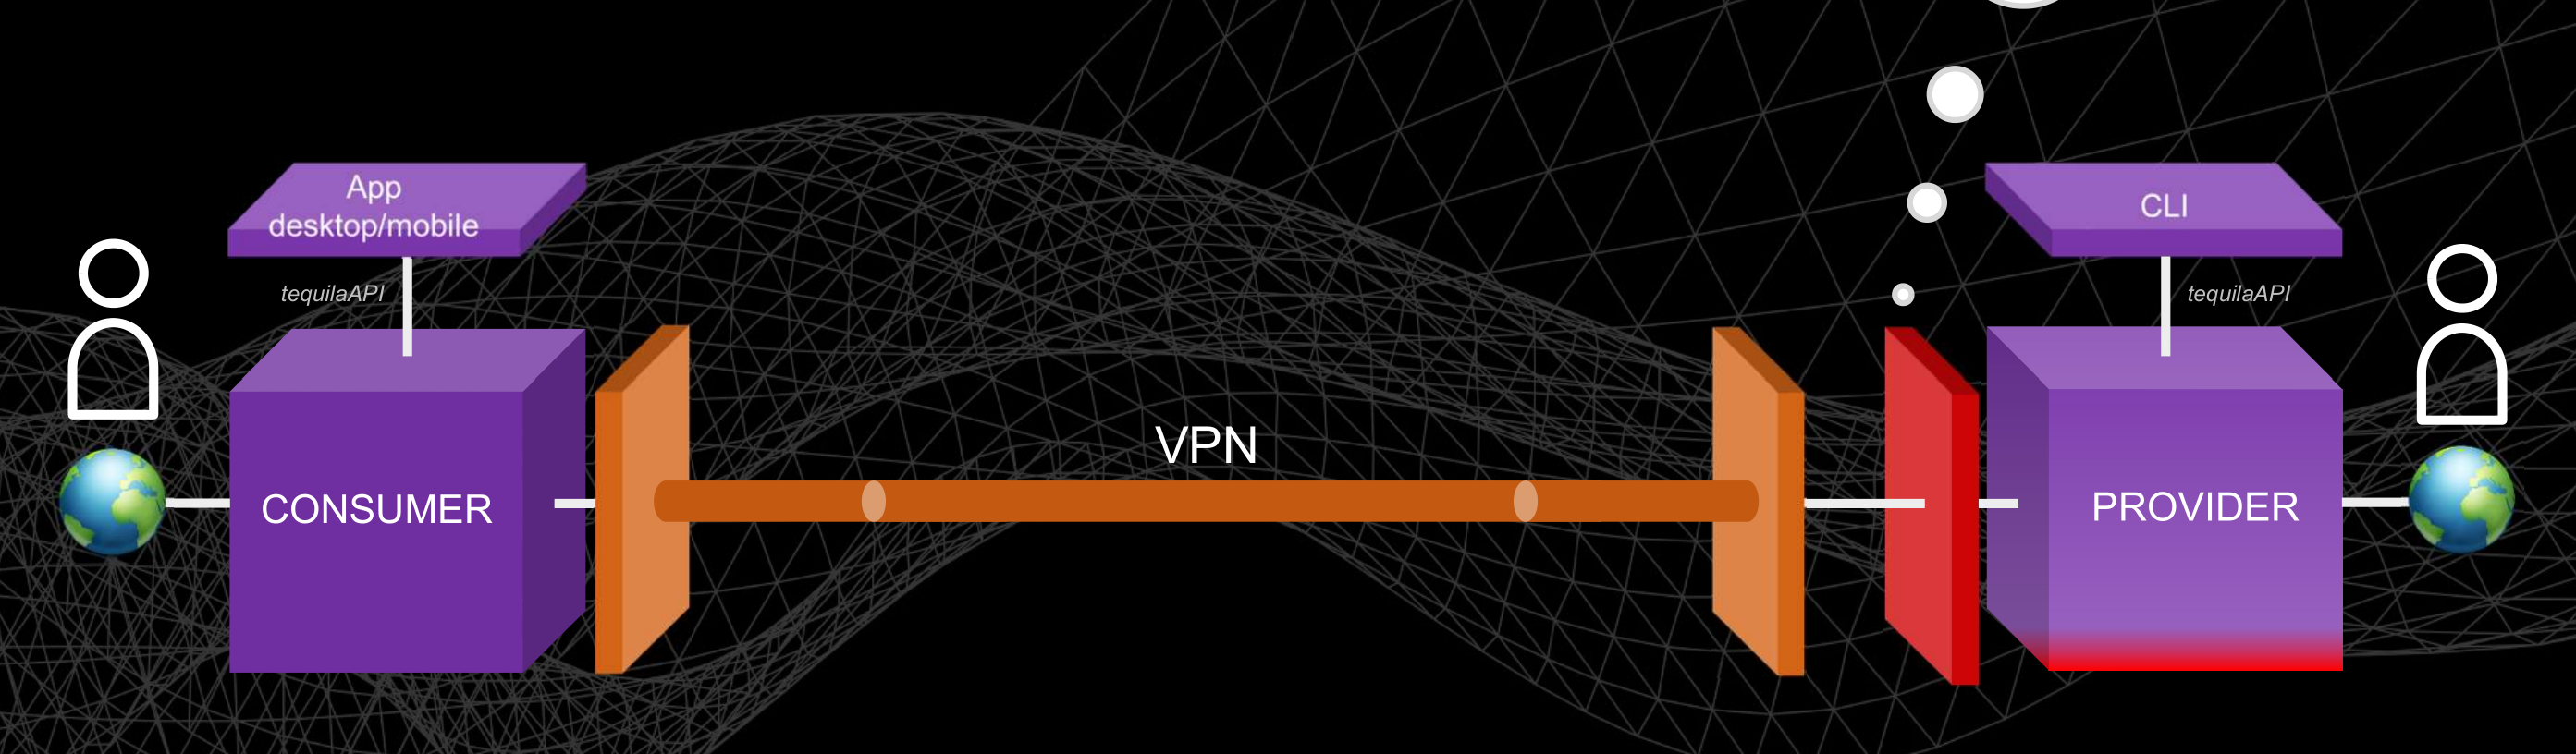
\includegraphics[width=\linewidth]{"images/client_server_vpn_connection.png"}



	\subsection{Basic sniffing to catch content (Wireshark, tcpdump)}
	Note:
	\begin{itemize}
		\item https://www.digitalocean.com/community/tutorials/a-deep-dive-into-iptables-and-netfilter-architecture
		\item http://linux-training.be/networking/ch14.html
	\end{itemize}
	
	\subsection{Craftberry, a demo tool}
			useful tips
			\begin{verbatim}
				http://unixwiz.net/techtips/gnu-c-attributes.html
				https://gcc.gnu.org/onlinedocs/gcc-4.0.2/gcc/Type-Attributes.html
				https://groups.google.com/forum/#!msg/pcapplusplus-support/e7rN93LfTSg/MFnVEKCNCAAJ
				https://byt3bl33d3r.github.io/using-nfqueue-with-python-the-right-way.html
			\end{verbatim}
			
			\subsubsection{liv 2: arp, vlan tagging}
			\subsubsection{liv 3: ip, icmp}
			\subsubsection{liv 4: tcp/udp}
			\subsubsection{side attacks}
				- auditin/collezione dei dati sniffati, inviati ad un server esterno per collezionamento, statistiche, vendita a terzi.
				- trojan all'interno di craftberry, per botnet. (approfondire aspetto che se il sw di attacco diventa popolare, può essere lui stesso veicolo di malware, quindi attacco l' attaccante)
			
			\begin{itemize}
				\item copia x volte dei pacchetti (TCP/UDP)
				\item gonfiamento dei pacchetti nei campi che poi verranno corretti dai check (TCP/UDP)
				\item modifica del payload se in chiaro (TCP/UDP)
				\item azione positiva sul payload (UDP), ad esempio cifratura chacha20
			\end{itemize}
		 	\subsubsection{liv 5+: http/imap/dns/ntp/etc}
				analisi e modifica dei contenuti a livello del singolo protocollo (ad esempio sostituzione di tutte le immagini con una immagine di default)
			
	\subsection{Tests}
	\subsection{Design solutions for malicious context}
		\subsubsection{comparing data}
		invia la richiesta a due nodi e le confronta (essenziale possibilità di connessione a due nodi in contemporanea: due o più container docker mappati su porte diverse con uno script che invia la richiesta a più container e confronta le risposte)

		\subsubsection{comparing hashes}
		come precedente ma con la gestione degli hash invece che di tutto il dato


	\subsection{Design integration with reputation systems}

		
\section{Conclusions}
	\subsection{Future development}
	\subsection{Considerations}

	The use of Mysterium Network like an end-to-end encryption tool: https://nakedsecurity.sophos.com/2015/06/25/can-you-trust-tors-exit-nodes/
	Here there is a nice consideration on how bad is an exit point for TOR.

	\pagebreak

	\textbf{problemi individuati}
	\begin{enumerate}
		\item valutazione della reputazione dell'agent da parte del client
		\item valutazione della reputazione dell'agent da parte della Net
	\end{enumerate}
	
	\textbf{soluzioni proposta}
	\textbf{Proposte per la valutazione della reputazione dell'agent da parte del client}
	
	Le seguenti proposte sono metodi di verifica del corretto comportamento ed hanno come scopo finale la valutazione della reputazione degli agent
	\begin{itemize}
		\item Dati civetta: modifiche al client che con scadenze richiede una o più risorse dal valore noto e verifica che siano integre. Le scadenze possono essere regolari/random/all’inizio frequenti/dipendenti dalla reputazione dell’agent. È necessario avere delle risorse distribuite e disponibili: potrebbero essere i nodi stessi della rete (altri agent).
		\item Dati duplicati: modifiche al client che implementa la possibilità di connessione con più agent. Dopo la richiesta il client compara i dati ottenuti dalle due fonti
		\begin{itemize}
			\item Hash *: (soluzione aggiuntiva) I nodi sono generalmente in posizioni migliori dei client in termini di velocità. L’idea è quella di far generare un hash dei dati che il client richiede ad un altro nodo fuori dal servizio primario, così da comparare gli hash e non tutto il dato.
			Inoltre, se la richiesta la faccio a molti più nodi posso intrinsicamente verificare quali modificano i dati nel network.
		\end{itemize}
		\item Applicazione di modelli di reputazione (Eigentrust): attualmente non studiato
	\end{itemize}

	\bibliographystyle{plain}
	\begin{thebibliography}{1}
		\bibitem{HTTPS}
			https://tools.ietf.org/html/rfc2818
		\bibitem{VPNRFC}
			https://tools.ietf.org/html/rfc2764
		\bibitem{wikibook}
			manually managing references, 
			\url{https://en.wikibooks.org/wiki/LaTeX/Manually_Managing_References}
			2016
		\bibitem{tc}
			traffic control
			https://jvns.ca/blog/2017/04/01/slow-down-your-internet-with-tc/
		\bibitem{exitnodeTOR}
			exit node TOR network
			https://www.wired.com/2007/09/rogue-nodes-turn-tor-anonymizer-into-eavesdroppers-paradise/?currentPage=all

	\end{thebibliography}
		
	\pagebreak
	
	%%	{\Large Valutazione di un nuovo utente della rete}
	\paragraph{Contesto}
	Rete VPN decentralizzata attiva e con connessione multi-hop tra una generica coppia Agent-Client.
	
	\paragraph{Problema 1: identificare gli Agent in posizione endnode che inviano contenuto non originale}
	In una rete VPN decentralizzata gli Agent endnode hanno il compito di recuperare una risorsa web e restituirla al Client attraverso la rete VPN instaurata. L'Agent, che quindi ha accesso intrinseco al dato ottenuto, cifrato o meno, può modificarlo prima di inviarlo al Client. Questa operazione può avere scopi malevoli, tra cui quello del guadagno economico. In possibile scenario, in questo contesto, è quello che vede l'incremento della grandezza del pacchetto da Agent a Client al fine di maggiorare i consumi della banda stabilita nel contratto iniziale di fornitura del servizio.
	
	\paragraph{Problema 2: scoraggiare abusi della rete}
	Per scoraggiare abusi della rete si utilizza una \textit{prova di lavoro} (Proof of Work) per attestare che il nuovo utente della rete ha speso delle risorse al fine di guadagnare reputazione nel contesto distruibuito.\\
	La reputazione iniziale, all'ingresso della rete distribuita, ha valore zero.
	
	\paragraph{Soluzione problema 1}
	\begin{itemize}
		\item Dati civetta: è richiesta dal Client all'Agent, con frequenza variabile, una risorsa dal valore noto al Client per la verifica di integrità. Se il test risulta negativo si ipotizza la modifica della risorsa da parte dell'Agent.
		\item Dati duplicati: il Client si connette a due Agent diversi e chiede ad entrambi la risorsa desiderata, alla ricezione si comparano per la verifica di integrità. Se il test risulta negativo si ipotizza la modifica della risorsa da parte di uno dei due Agent.\\
		\textbf{Aspetti negativi:} questa soluzione non è applicabile in caso di connessioni con la risorsa che prevedono \textit{stati}.(??)
		\item Hash Dato: il Client si connette ad un Agent al quale chiede una risorsa e successivamente chiede ad un altro Agent l'hash della risorsa stessa. Il Client effettua quindi un hash (stessa funzione hash) della risorsa ottenuta dall'Agent e la compara con l'hash ottenuto dal secondo Agent. Ulteriore implementazione può essere effettuata richiedendo a più agent l'hash della risorsa.\\
		Se il test risulta negativo si ipotizza la modifica della risorsa da parte del primo Agent.\\
		\textbf{Aspetti negativi:} questa soluzione non è applicabile in caso di connessioni con la risorsa che prevedono \textit{stati}.\\
		\textbf{Caso d'uso:} si reputa questo metodo adatto a verificare un Agent al suo primo ingresso nella rete in quanto non è spesso adatto per l'aspetto negativo sopra descritto.		
	\end{itemize}
	
	\paragraph{Soluzione problema 2}
	L'originalità della soluzione proposta è l'operazione di Proof of Work da far compiere al nuovo utente. Si propone come prova di lavoro che l'utente, prima di entrare attivamente a far parte della rete o durante la sua partecipazione, consumi della banda internet.\\
	La Proof of Work, quindi, consiste nello sfruttare la sua banda internet per ottenere una risorsa internet, sulla quale viene verificata l'integrità, come descritto nella soluzione \textit{Dato Hash} proposta nella soluzione al problema 1.\\ 
	Più specificatamente, nel caso d'uso si identificano un Agent A, un Client C ed un nuovo utente X che vuole entrare nella rete e deve dimostrare \textit{la prova di lavoro}.\\
	La situazione iniziale prevede una connessione tra A e C. Per verificare che A fornisca dato $d^A$ originale, C richiede a X di ottenere lo stesso dato $d^X$ e di eseguirne la funzione hash così da ottenere  $H(d^X)=h_1$. $h_1$ sarà restituito a C che ha già effettuato la stessa funzione hash su $d^A$ proveniente da A ed ha ottenuto $H(d^A) = h_2$.\\
	Il test di integrità verifica che $h_1 = h_2$.\\
	Se il test ha successo si ha certezza che:
	\begin{enumerate}
		\item il nuovo utente X ha eseguito correttamente la proof of work 
		\item A ha fornito a C un dato originale, a meno che sia A che X applichino le stesse modifiche al dato prima di effettuarne la funzione hash.\\Questa vincolo è da verificare.
	\end{enumerate}
	
	\paragraph{Considerazioni}
	In un contesto di rete distribuita si possono ipotizzare $n$ attori nel ruolo di X e $n$ test di integrità che C effettua per verificare l'integrità del dato ottenuto da A. \textit{riferimento al consenso BFT}\\
	Il risultato dei test condiziona la reputazione di ogni attore nel ruolo di $X$.\\
	Si può ipotizzare l'applicazione della soluzione $m$ volte, tante quante sono le entità per cui effettuare la proof of work, e considere vincoli come tempo $t$ minimo di esecuzione della proof of work o la quantità minima di dati $q$ che $X$ deve ottenere su cui applicare la funzione hash.\\
	
	
	Considerando una costo ipotetico $c$ associato al consumo di una quantità $q$ di dati per un'unità di tempo $t$ si può impostare una soglia $S = c*q*t$ superata la quale la proof of work si può considerare eseguita.\\
	L'ultima affermazione garantisce l'asimmetria della proof of work (??). (che è: hash difficile da calcolare perchè spendo risorsa di tempo e di banda e facile da verificare dal client perchè effettuo un semplice confronto di un hash)(vedere https://it.wikipedia.org/wiki/Hashcash per similitudini sulla variabile del tempo)\\
	
	
	La reputazione di ogni entità all'interno della rete, sia Agent che Client, subisce una variazione in quanto ciascun esito delle proof of work viene registrata nella blockchain e questo consente di avere una classifica di affidabilità delle entità quasi in tempo reale.\\
	

	

\end{document}